\documentclass[a4paper, 11pt]{article}
\usepackage{comment}
\usepackage{fullpage}
\usepackage{amsmath}
\usepackage{amssymb}
\usepackage{mathtools}
\usepackage{fontspec}
\usepackage{siunitx}
\defaultfontfeatures{Ligatures=TeX}
\usepackage{xfrac}
\usepackage{icomma}
\usepackage[section,below]{placeins}
\usepackage[labelfont=bf,font=small,width=0.9\textwidth]{caption}
\usepackage{subcaption}
\usepackage{graphicx}
\usepackage{grffile}
\usepackage{float}
\floatplacement{figure}{htbp}
\floatplacement{table}{htbp}
\usepackage{booktabs}
\usepackage{hyperref}
\begin{document}
\noindent
\centerline{\small{\textsc{Michigan State University}}} \\
\large{\textbf{CMSE/CSE 822 – Parallel Computing \hfill Fall 2019 \\
Homework 2}} \\
Alexander Harnisch \\
\noindent\makebox[\linewidth]{\rule{\textwidth}{0.4pt}}

\section*{1) Performance Modeling}
\subsection*{a)}
\label{sec:1a}
There is some missing information here and assumptions have to be made.
However, it's not important since it only effects the numbers to plug in and
get out, not the logic behind it.

The kernel performs 6 floating point operations (FLOP) in each iteration.
Assuming no caching we have seven floating point number reading and one writing
operation for each loop iterations. Assuming single precision with
$\SI{4}{byte}$ per float that translates to $\SI{32}{byte}$ of memory acces and
an arithmetic intensity $I$ of
\begin{equation}
  I = \frac{\SI{6}{FLOP}}{\SI{32}{byte}} = \frac{3}{16}\,\frac{\textup{FLOP}}{\textup{byte}}\,.
\end{equation}
For double precision we obviously get half of that. Assuming some caching where
at least the same variable has to be loaded only once per loop iteration, we
would have just 2 reading operations and therefore $\SI{8}{byte}$ of memory
access which would result in $I = \SI{3/4}{FLOP\per byte}$ for single and half
that for double precision. Depending on many factors (caching, compiler used,
etc.) the actual numbers might be different.

\subsection*{b)}
In a simple roofline model for some $I$ the critical peak performance
$\pi_\textup{crit}$ is given by $\beta I$, where $\beta$ is the peak memmory
bandwith. So whatever the assumptions and resulting $I$ from
\hyperref[sec:1a]{a)} is, for a peak performance of larger than
$\pi_\textup{crit}$ the kernel would be compute bound, otherwise memory bound.

Let's say we have double precision and some caching, so $I = \frac{3}{8}\,\frac{\textup{FLOP}}{\textup{byte}}$ we would get
\begin{equation}
  \pi_\textup{crit} = 30\,\frac{\textup{GB}}{\textup{s}}\cdot \frac{3}{8}\,\frac{\textup{FLOP}}{\textup{byte}} = 11.25\,\frac{\textup{GFLOP}}{\textup{s}}\,.
\end{equation}

\newpage
\subsection*{c)}
A simple roofline model plot is given by Figure~\ref{fig:roofline}. The
performance for an arithmetic intensity of $I = \SI{3/8}{FLOP\per byte}$ is
$\SI{11.25}{GFLOP\per\second}$.
\begin{figure}
  \centering
  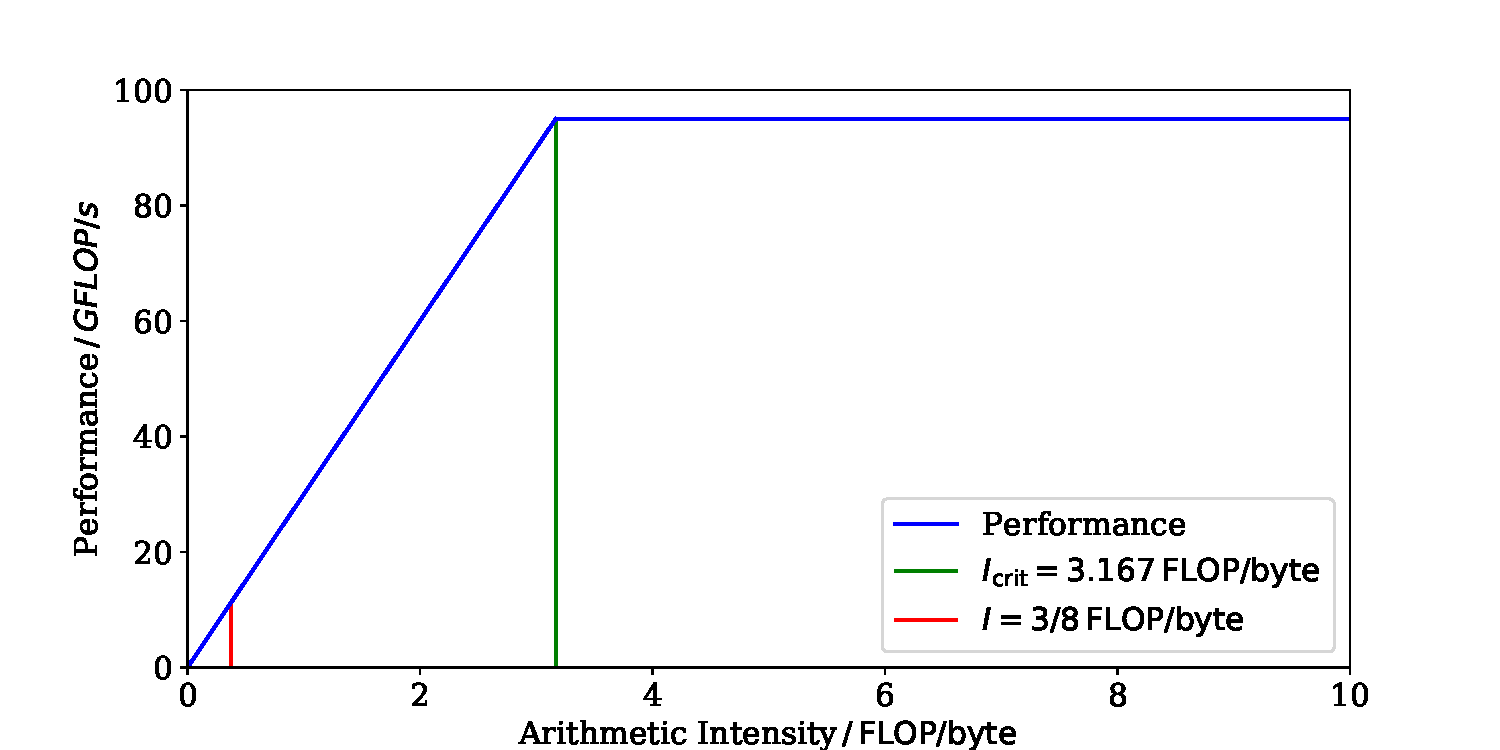
\includegraphics[width=\textwidth]{../plot/roofline.pdf}
  \caption{Simple roofline model.}
  \label{fig:roofline}
\end{figure}

\section*{2) Cache optimization: Matrix Vector Multiplication}


\end{document}
